\documentclass[a4paper]{article}
\usepackage{lmodern}
\usepackage{amssymb,amsmath}
\usepackage{ifxetex,ifluatex}
\usepackage{fixltx2e} % provides \textsubscript
\ifnum 0\ifxetex 1\fi\ifluatex 1\fi=0 % if pdftex
  \usepackage[T1]{fontenc}
  \usepackage[utf8]{inputenc}
\else % if luatex or xelatex
  \ifxetex
    \usepackage{mathspec}
  \else
    \usepackage{fontspec}
  \fi
  \defaultfontfeatures{Ligatures=TeX,Scale=MatchLowercase}
\fi
% use upquote if available, for straight quotes in verbatim environments
\IfFileExists{upquote.sty}{\usepackage{upquote}}{}
% use microtype if available
\IfFileExists{microtype.sty}{%
\usepackage{microtype}
\UseMicrotypeSet[protrusion]{basicmath} % disable protrusion for tt fonts
}{}
\usepackage[margin=1in]{geometry}
\usepackage{hyperref}
\hypersetup{unicode=true,
            pdftitle={Project 2},
            pdfauthor={Axel Sjöberg \& John Rapp Farnes},
            pdfborder={0 0 0},
            breaklinks=true}
\urlstyle{same}  % don't use monospace font for urls
\usepackage{longtable,booktabs}
\usepackage{graphicx,grffile}
\makeatletter
\def\maxwidth{\ifdim\Gin@nat@width>\linewidth\linewidth\else\Gin@nat@width\fi}
\def\maxheight{\ifdim\Gin@nat@height>\textheight\textheight\else\Gin@nat@height\fi}
\makeatother
% Scale images if necessary, so that they will not overflow the page
% margins by default, and it is still possible to overwrite the defaults
% using explicit options in \includegraphics[width, height, ...]{}
\setkeys{Gin}{width=\maxwidth,height=\maxheight,keepaspectratio}
\IfFileExists{parskip.sty}{%
\usepackage{parskip}
}{% else
\setlength{\parindent}{0pt}
\setlength{\parskip}{6pt plus 2pt minus 1pt}
}
\setlength{\emergencystretch}{3em}  % prevent overfull lines
\providecommand{\tightlist}{%
  \setlength{\itemsep}{0pt}\setlength{\parskip}{0pt}}
\setcounter{secnumdepth}{5}
% Redefines (sub)paragraphs to behave more like sections
\ifx\paragraph\undefined\else
\let\oldparagraph\paragraph
\renewcommand{\paragraph}[1]{\oldparagraph{#1}\mbox{}}
\fi
\ifx\subparagraph\undefined\else
\let\oldsubparagraph\subparagraph
\renewcommand{\subparagraph}[1]{\oldsubparagraph{#1}\mbox{}}
\fi

%%% Use protect on footnotes to avoid problems with footnotes in titles
\let\rmarkdownfootnote\footnote%
\def\footnote{\protect\rmarkdownfootnote}

%%% Change title format to be more compact
\usepackage{titling}

% Create subtitle command for use in maketitle
\providecommand{\subtitle}[1]{
  \posttitle{
    \begin{center}\large#1\end{center}
    }
}

\setlength{\droptitle}{-2em}

  \title{Project 2}
    \pretitle{\vspace{\droptitle}\centering\huge}
  \posttitle{\par}
    \author{Axel Sjöberg \& John Rapp Farnes}
    \preauthor{\centering\large\emph}
  \postauthor{\par}
      \predate{\centering\large\emph}
  \postdate{\par}
    \date{14 maj 2019}


\begin{document}
\maketitle

{
\setcounter{tocdepth}{3}
\tableofcontents
}
\newpage

\hypertarget{introduction}{%
\section{Introduction}\label{introduction}}

\hypertarget{background-and-dataset}{%
\subsection{Background and dataset}\label{background-and-dataset}}

The objective of this report was to determine which covarites that can
be used to predict if a US county has a low or high crime rate (per 1000
inhabitants). Data used to do this was county demographic information
(CDI) for 440 of the most populous counites in the US 1990-1992. The
record for each county includes data on the 14 variables listed below in
table \ref{tab:cdi}. Counties with missing data has been removed from
the dataset.

\begin{longtable}[]{@{}ll@{}}
\caption{\label{tab:cd}iCDI dataset columns}\tabularnewline
\toprule
Variable & Description\tabularnewline
\midrule
\endfirsthead
\toprule
Variable & Description\tabularnewline
\midrule
\endhead
id & identification number, 1--440\tabularnewline
county & county name\tabularnewline
state & state abbreviation\tabularnewline
area & land area (square miles)\tabularnewline
popul & estimated 1990 population\tabularnewline
pop1834 & percent of 1990 CDI population aged 18--34\tabularnewline
pop65plus & percent of 1990 CDI population aged 65 years old or
older\tabularnewline
phys & number of professionally active nonfederal physicians during
1990\tabularnewline
beds & total number of beds, cribs and bassinets during
1990\tabularnewline
crimes & total number of serious crimes in 1990\tabularnewline
higrads & percent of adults (25 yrs old or older) who completed at least
12 years of school\tabularnewline
bachelors & percent of adults (25 yrs old or older) with bachelor's
degree\tabularnewline
poors & Percent of 1990 CDI population with income below poverty
level\tabularnewline
unemployed & percent of 1990 CDI labor force which is
unemployed\tabularnewline
percapitaincome & per capita income of 1990 CDI population
(dollars)\tabularnewline
totalincome & total personal income of 1990 CDI population (in millions
of dollars)\tabularnewline
region & Geographic region classification used by the U.S. Bureau of the
Census,\tabularnewline
& including Northeast, Midwest, South and West\tabularnewline
\bottomrule
\end{longtable}

In order to measure crime rate, another varible called \texttt{crm1000}
was added to the data set, descibing the number of serious crimes per
1000 inhabitants. Same thing with \texttt{phys}, with \texttt{phys1000}.
Using \texttt{crm1000}, counties were divided into counties with high or
non-high crime rate, using the median of \texttt{crm1000}, where
counties with crime rate higher than the median were categorized as
having a high crime rate. This crime status of the county was stored in
another column called \texttt{hircrm}, which takes the value 1 if the
county is a high crime county and zero if it is a low crime county. In
this paper, this binary varible will be used as the dependent varible.
This binary dependent value was then modelled using
\textbf{logistic regression}.

\hypertarget{model}{%
\subsection{Model}\label{model}}

The logistic regression model used, models the log-odds of a certain
observation \(i\) as a linear combination of its covariates \(X_{j,i}\)
and parameters \(\beta_i\), with together with an additive error
\(\epsilon_i\). These error terms are assumed to follow a normal
distribution and be indipendent, i.e.~\(\epsilon \sim N(0, \sigma)\)
i.i.d. \begin{equation}
  \ln{\frac{p_i}{1 - p_i}} = \beta_0 + \sum_j\beta_{j} \cdot X_{j,i} + \epsilon_i
\end{equation}

\hypertarget{analysis}{%
\section{Analysis}\label{analysis}}

\hypertarget{the-higrad-model}{%
\subsection{The higrad model}\label{the-higrad-model}}

\hypertarget{introduction-1}{%
\subsubsection{Introduction}\label{introduction-1}}

The model becomes

\begin{equation}
  \ln{\frac{p_i}{1 - p_i}} = \beta_0 + \beta_{higrads} \cdot X_{higrads,i} + \epsilon_i
\end{equation}

The first model considered had \texttt{higrads} as the sole covariate.
In order to determine if there is a relationship between \texttt{hicrm}
and \texttt{higrads} they are plotted against each other, see figure
\ref{fig:hicrm_higrads}. Because \texttt{hicrm} is a binary varible it
is very difficult to determine if there is a relationship by the pattern
of the plot. In order to circumvent this problem a kernel smoother was
added to the plot. The most smooth looking line was attained by setting
the bandwidth to 20. The kernel curve was sort of S-shaped, implying
that a logistic model may be appropriate. Further, the S-shape is
``downward facing'', implying a negative \(\beta_{higrads}\), as the
probability of a county being classified as a high crime county
decreases when the amount of higrads in the county increses. Furthermore
the fitted model along with its 95 \% confidence interval was added to
the plot in figure \ref{fig:hicrm_higrads}.

\begin{figure}[h]
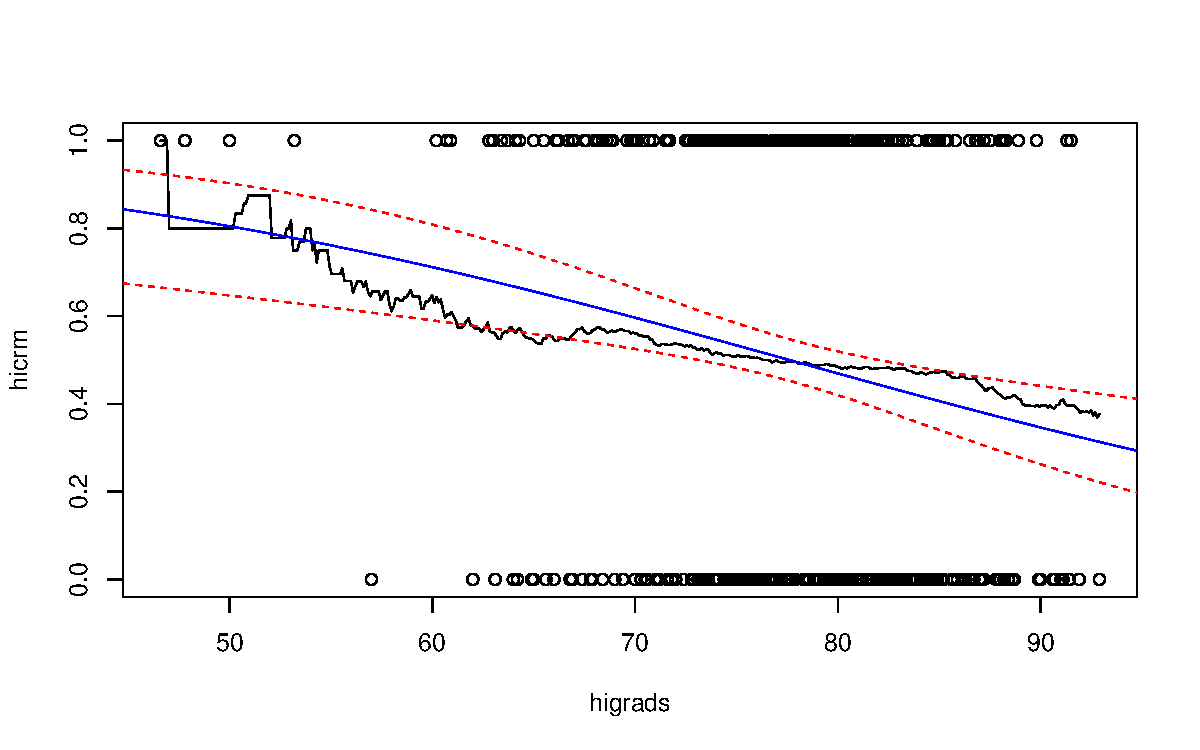
\includegraphics{Project_2_files/figure-latex/unnamed-chunk-2-1} \caption{\label{fig:hicrm_higrads}Plot of \texttt{hicrm} against \texttt{higrads}, including kernel smoothing and prediction of fitted model with 95 \% confidence interval}\label{fig:unnamed-chunk-2}
\end{figure}

NÅGOT OM ATT DEN INTE BESKRIVER JÄTTEBRA, BARA FRÅN 60\% till 40\% DÄR
DET FINNS DATA?

As can be seen in figure \ref{fig:hicrm_higrads}, a higher number of
`higrads seems to make a county less probable to qualify as high crime
county. Logically this makes sense. Tee \(\beta\) values together with
their 95 \% confidence inteval is presented in table
\ref{tab:higrad_beta}. Neither one of the \(\beta\) confidence interval
cover zero, meaning that they are statistically significant at
\(\alpha\) = 0.05. This is verfied by the very small P value. Something
concerning about the plot in figure 1 is the few data point to the
middle of the left, as they might influence predicted model in an
erronious manner. Moreover the interval covered by the kernel smoother
and the predicited model is quite low.

\hypertarget{fitted-model-and-significance}{%
\subsubsection{Fitted model and
significance}\label{fitted-model-and-significance}}

\begin{longtable}[]{@{}lrrrr@{}}
\caption{\label{tab:higrad_beta}\(\beta\)-values of \texttt{higrad}
model, with 95 \% confidence inteval}\tabularnewline
\toprule
& Estimate & 2.5 \% & 97.5 \% & P-value\tabularnewline
\midrule
\endfirsthead
\toprule
& Estimate & 2.5 \% & 97.5 \% & P-value\tabularnewline
\midrule
\endhead
\(\beta_0\) & 3.980 & 1.805 & 6.250 & 0.00044\tabularnewline
\(\beta_{higrads}\) & -0.051 & -0.080 & -0.023 & 0.00041\tabularnewline
\bottomrule
\end{longtable}

If higrads increases 1\%, odd decreases by 5\% If higrads increases
10\%, odd decreases by 40.1\%

\hypertarget{model-predictions}{%
\subsubsection{Model predictions}\label{model-predictions}}

Using the higrads model,the probability, with confidence interval, of
having a high crime rate in a county where the amount of higrads is 65
(percent), and where it is 85 (percent) is predicted. The result can be
found in table 3.

\begin{longtable}[]{@{}rrrr@{}}
\caption{Test}\tabularnewline
\toprule
Higrads & Probability (\%) & 2.5 \% & 97.5 \%\tabularnewline
\midrule
\endfirsthead
\toprule
Higrads & Probability (\%) & 2.5 \% & 97.5 \%\tabularnewline
\midrule
\endhead
6500 & 65.6 & 55.9 & 74.2\tabularnewline
8500 & 40.6 & 34.1 & 47.6\tabularnewline
\bottomrule
\end{longtable}

\hypertarget{model-performance-analysis}{%
\subsubsection{Model performance
analysis}\label{model-performance-analysis}}

In order to analyze model performance, the sensitivity and specificity
of the model was calculated. The sensitivity of a model is the ratio of
predicted positives to real positives in the dataset, while the
specificity of a model is the ratio of predicted negatives to real
negatives in the dataset. As such, the higher the value of the
sensitivity and specificity, the better.

The sensitivity of the model was 55.5\% and specificity of the model was
57.3\%. Thereby the higrad model does a rather bad job at correctly
clasifying the the crime level status of the counties

\hypertarget{the-region-model}{%
\subsection{The region model}\label{the-region-model}}

\hypertarget{introduction-2}{%
\subsubsection{Introduction}\label{introduction-2}}

Next, a logistic model was adopted based on \texttt{region}. Since
\texttt{region} is not continous , but categorial, it is modelled using
``dummy variables'' \(X_i\). In order to implement this effectively, one
of the categories is chosen as a reference variable, and the effects of
other categories are measured in comparison to it.

In order to determine this reference variable - a cross-tabulation of
the data between \texttt{region} and \texttt{hirm} is studied, see table
\ref{tab:cross-tabulation}.

\begin{longtable}[]{@{}lrr@{}}
\caption{\label{tab:cross-tabulation}Cross-tabulation between
\texttt{region} and \texttt{hicrm}}\tabularnewline
\toprule
& Low crime & High crime\tabularnewline
\midrule
\endfirsthead
\toprule
& Low crime & High crime\tabularnewline
\midrule
\endhead
Northeast & 82 & 21\tabularnewline
Midwest & 64 & 44\tabularnewline
South & 44 & 108\tabularnewline
West & 30 & 47\tabularnewline
\bottomrule
\end{longtable}

As a reference region, the one that has the largest number of counties
in it's smallest low/high category was chosen. As a tie-breaker, the
other low/high category was used. This approach produces the lowest
standard error, and therefore highest significance. As seen in table
\ref{tab:cross-tabulation}, the above given condition results in
choosing South as reference region.

Using this reference region, the logistic model becomes \begin{equation}
  \ln{\frac{p_i}{1 - p_i}} = \beta_0 + \beta_{Northeast} \cdot X_{Northeast,i} + \beta_{Midwest} \cdot X_{Midwest,i} + \beta_{West} \cdot X_{West,i} + \epsilon_i
\end{equation}

The \(\beta\) coefficients are measured relative to South and
\(\beta_0\) is log-odds coefficient for South.

\hypertarget{fitted-model-and-significance-1}{%
\subsubsection{Fitted model and
significance}\label{fitted-model-and-significance-1}}

The model was fit with the given data set, estimating \(\beta_i\), shown
together with its 95 \% confidence interval and P-value, in table
\ref{tab:region_beta}.

\begin{longtable}[]{@{}lrrrr@{}}
\caption{\label{tab:region_beta}\(\beta\)-estimates for the
\texttt{region} model, together with 95 \% confidence interval and
P-values}\tabularnewline
\toprule
& Estimate & 2.5 \% & 97.5 \% & P-value\tabularnewline
\midrule
\endfirsthead
\toprule
& Estimate & 2.5 \% & 97.5 \% & P-value\tabularnewline
\midrule
\endhead
\(\beta_0\) & 0.898 & 0.555 & 1.258 & 0.000\tabularnewline
\(\beta_{Northeast}\) & -2.260 & -2.874 & -1.682 & 0.000\tabularnewline
\(\beta_{Midwest}\) & -1.273 & -1.800 & -0.758 & 0.000\tabularnewline
\(\beta_{West}\) & -0.449 & -1.025 & 0.131 & 0.127\tabularnewline
\bottomrule
\end{longtable}

As may be seen in \ref{tab:region_beta}, the P-values for all of the
\(\beta\)-estimates are not less than 0.05, indicating a lack of
statistical significance on a 95 \% level. \(\beta_{west}\) is the only
varible that has a P-value \textgreater{} 0.05. This means that the west
region dummy varible might be irrelevant when having south as the
reference category.

Next, the odds-ratios for the different categories where determined. The
odds-ratios measure the odds of a particular category in relation to the
reference category. These may be calculated as \(OR_i = e^{\beta_i}\)
and are seen in table \ref{tab:region_OR}.

\begin{longtable}[]{@{}lrrr@{}}
\caption{\label{tab:region_OR}Odds-ratios for the \texttt{region} model,
together with 95 \% confidence interval}\tabularnewline
\toprule
& OR & 2.5 \% & 97.5 \%\tabularnewline
\midrule
\endfirsthead
\toprule
& OR & 2.5 \% & 97.5 \%\tabularnewline
\midrule
\endhead
Northeast & 0.10 & 0.06 & 0.19\tabularnewline
Midwest & 0.28 & 0.17 & 0.47\tabularnewline
West & 0.64 & 0.36 & 1.14\tabularnewline
\bottomrule
\end{longtable}

As seen in table \ref{tab:region_OR}, the odds-ratios are less than 1
for all categories but the reference region. This implies that the odds
for all regions are lower compared to the reference region, i.e.~that
the probability of a high crime rate is lower in all regions compared to
the reference region. This can also be seen in table
\ref{tab:cross-tabulation}.

\hypertarget{model-predictions-1}{%
\subsubsection{Model predictions}\label{model-predictions-1}}

Using the fitted model, the probabilies of having a high crime rate,
with confidence interval, for the different regions was determined,
shown in table \ref{tab:region_prob}.

\begin{longtable}[]{@{}lrrr@{}}
\caption{\label{tab:region_prob}Probability of high crime rate (\%),
together with 95 \% confidence interval for each of the
regions}\tabularnewline
\toprule
& Probability (\%) & 2.5 \% & 97.5 \%\tabularnewline
\midrule
\endfirsthead
\toprule
& Probability (\%) & 2.5 \% & 97.5 \%\tabularnewline
\midrule
\endhead
Northeast & 20.4 & 12.6 & 28.2\tabularnewline
Midwest & 40.7 & 31.5 & 50.0\tabularnewline
South & 71.1 & 63.8 & 78.3\tabularnewline
West & 61.0 & 50.1 & 71.9\tabularnewline
\bottomrule
\end{longtable}

\hypertarget{model-performance-analysis-1}{%
\subsubsection{Model performance
analysis}\label{model-performance-analysis-1}}

For the \texttt{region}, the sensitivity was 70.5\%, while the
specificity was 66.4\%.

Comparing the two models analyzed so far, the \texttt{region} model
performs better measured on sensitivity and specificity, as seen in
table \ref{tab:compare_sense_spec_region_higrad}

\begin{longtable}[]{@{}lrr@{}}
\caption{\label{tab:compare_sense_spec_region_higrad}Comparison of
sensitivity and specificity of \texttt{higrad} and \texttt{region}
model}\tabularnewline
\toprule
Covariate & Sensitivity (\%) & Specificity (\%)\tabularnewline
\midrule
\endfirsthead
\toprule
Covariate & Sensitivity (\%) & Specificity (\%)\tabularnewline
\midrule
\endhead
Higrads & 55.5 & 57.3\tabularnewline
Region & 70.5 & 66.4\tabularnewline
\bottomrule
\end{longtable}

\hypertarget{combined-model-and-comparison}{%
\subsection{Combined model and
comparison}\label{combined-model-and-comparison}}

\hypertarget{introduction-3}{%
\subsubsection{Introduction}\label{introduction-3}}

Next a model that uses both \texttt{higrads} and \texttt{region} is
analyzed. As such, this model becomes

\begin{equation}
  \ln{\frac{p_i}{1 - p_i}} = \beta_0 + \beta_{Northeast} \cdot X_{Northeast,i} + \beta_{Midwest} \cdot X_{Midwest,i} + \beta_{West} \cdot X_{West,i} + \beta_{higrads} \cdot X_{higrads,i} + \epsilon_i
\end{equation}

\hypertarget{model-comparison}{%
\subsubsection{Model comparison}\label{model-comparison}}

In order to compare the models, metrics other than sensitivity and
specificity may be studied. Some of these are AIC and BIC, which are
penalized-likelihood criteria and Nagelkerke psuedo \(R^2\), which is a
measurment that increses up to 1 the better the model fit is. As they
are defined, AIC and BIC should be as low as possible for a model to be
performant, while psuedo \(R^2\) should be as high as possible.

Comparison between the models in regards to AIC, BIC and Psuedo \(R^2\)
are seen in figure \ref{fig:comparison_region_higrads_both}, while
comparison of sensitivity and specificity is seen in table
\ref{tab:compare_sense_spec_region_higrad_both}.

\begin{figure}[h]
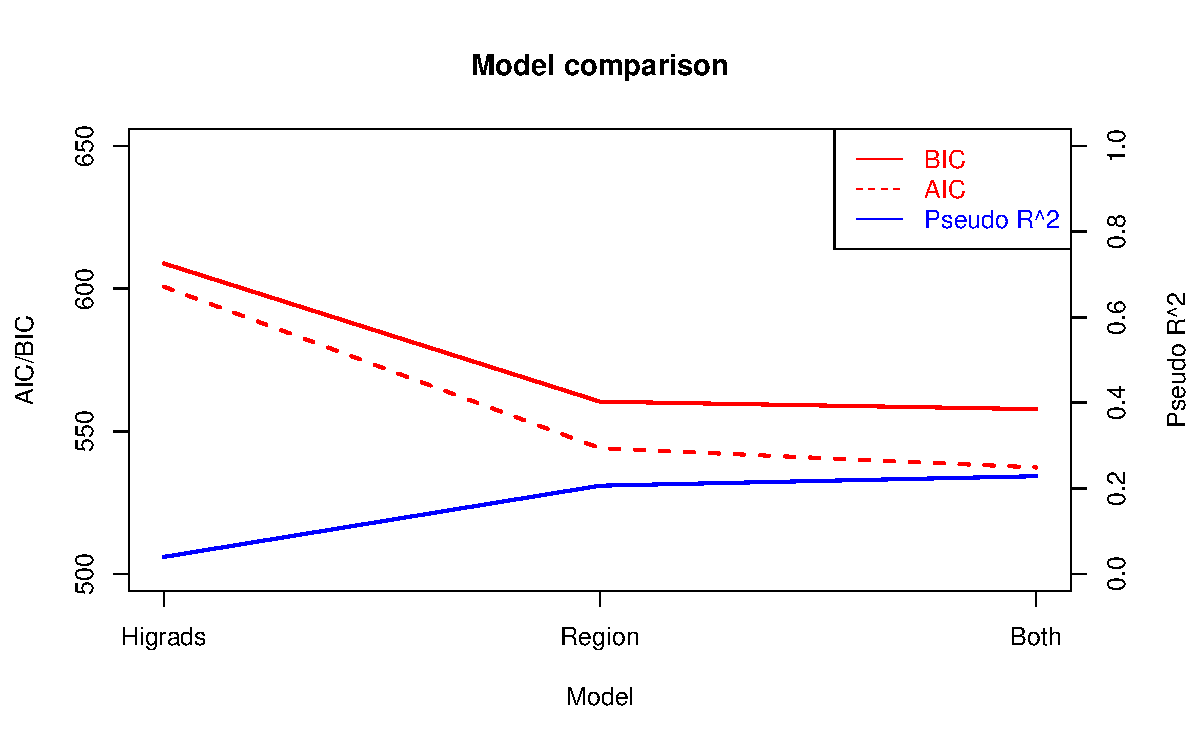
\includegraphics{Project_2_files/figure-latex/unnamed-chunk-8-1} \caption{\label{fig:comparison_region_higrads_both}Comparison of AIC and BIC and Nagelkerke psuedo $R^2$ for the different models}\label{fig:unnamed-chunk-8}
\end{figure}

\begin{longtable}[]{@{}lrr@{}}
\caption{\label{tab:compare_sense_spec_region_higrad_both}Comparison of
sensitivity and specificity of models}\tabularnewline
\toprule
Covariate & Sensitivity (\%) & Specificity (\%)\tabularnewline
\midrule
\endfirsthead
\toprule
Covariate & Sensitivity (\%) & Specificity (\%)\tabularnewline
\midrule
\endhead
Higrads & 55.5 & 57.3\tabularnewline
Region & 70.5 & 66.4\tabularnewline
Both & 70.5 & 67.3\tabularnewline
\bottomrule
\end{longtable}

As seen in figure \ref{fig:comparison_region_higrads_both} and table
\ref{tab:compare_sense_spec_region_higrad_both}, the combined model with
both the covariates performs the best on all the studied metrics.

\hypertarget{combined-model-performance}{%
\subsubsection{Combined model
performance}\label{combined-model-performance}}

Performance of the combined model can be analyzed by studying a QQ-plot
(see figure \ref{fig:qq-plot_combined}) the squared standardized Pearson
residuals and the standardized deviance residuals against the linear
predictor \(x^{\beta}\) (see figure \ref{fig:residuals_combined}). As
well as the Cook's distance against the linear predictor, and against
\texttt{higrads} and against \texttt{region} (see figure
\ref{fig:cooks_combined}).

\newpage

\begin{figure}[h]
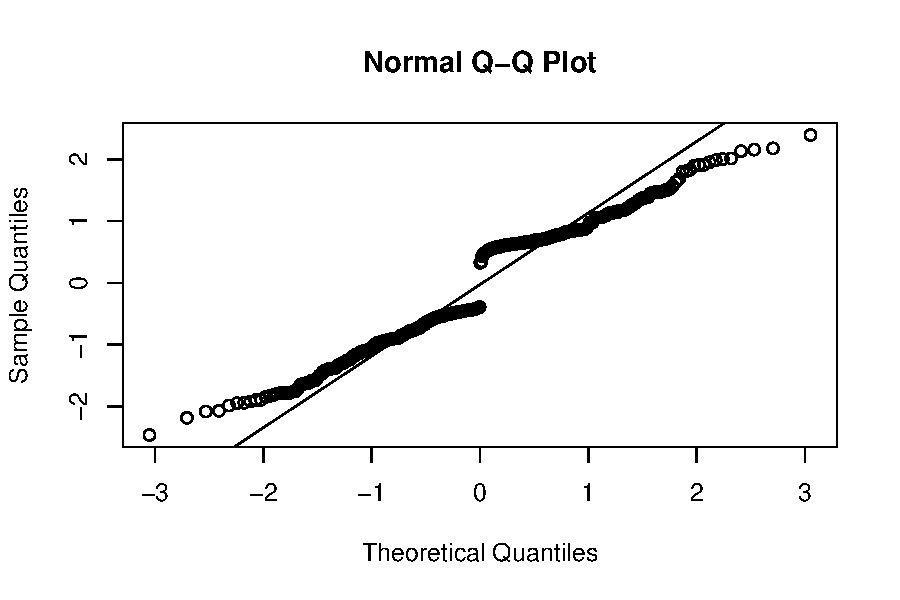
\includegraphics{Project_2_files/figure-latex/unnamed-chunk-10-1} \caption{\label{fig:qq-plot_combined}QQ-plot for the combined model}\label{fig:unnamed-chunk-10}
\end{figure}

The QQ-plot seem to follow a bimodal distribution.

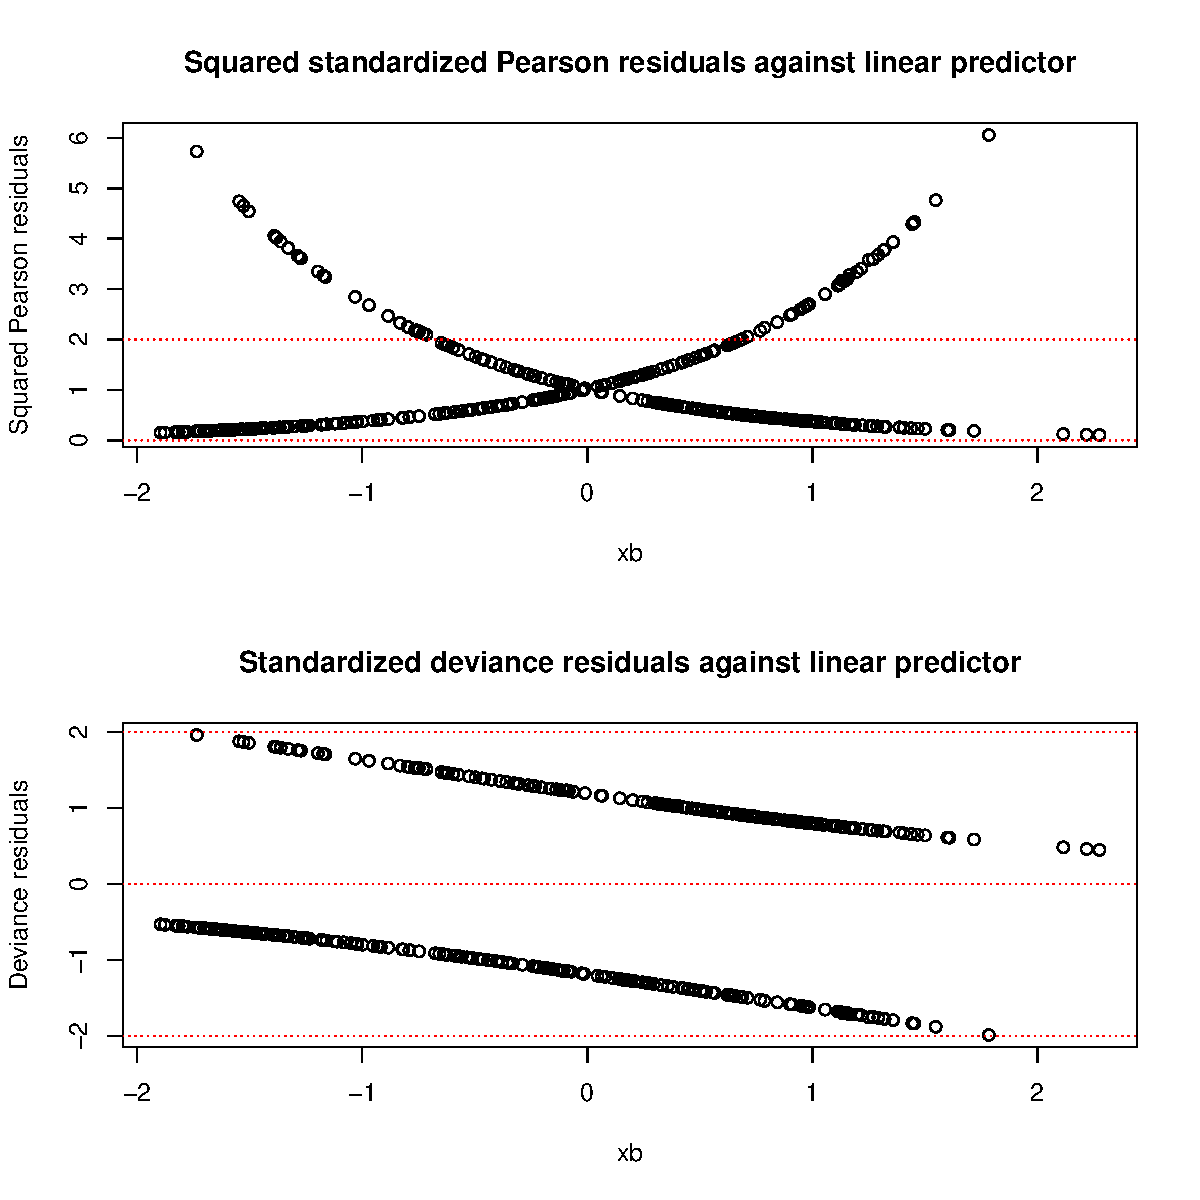
\includegraphics{Project_2_files/figure-latex/unnamed-chunk-11-1.pdf}

\begin{figure}[h]
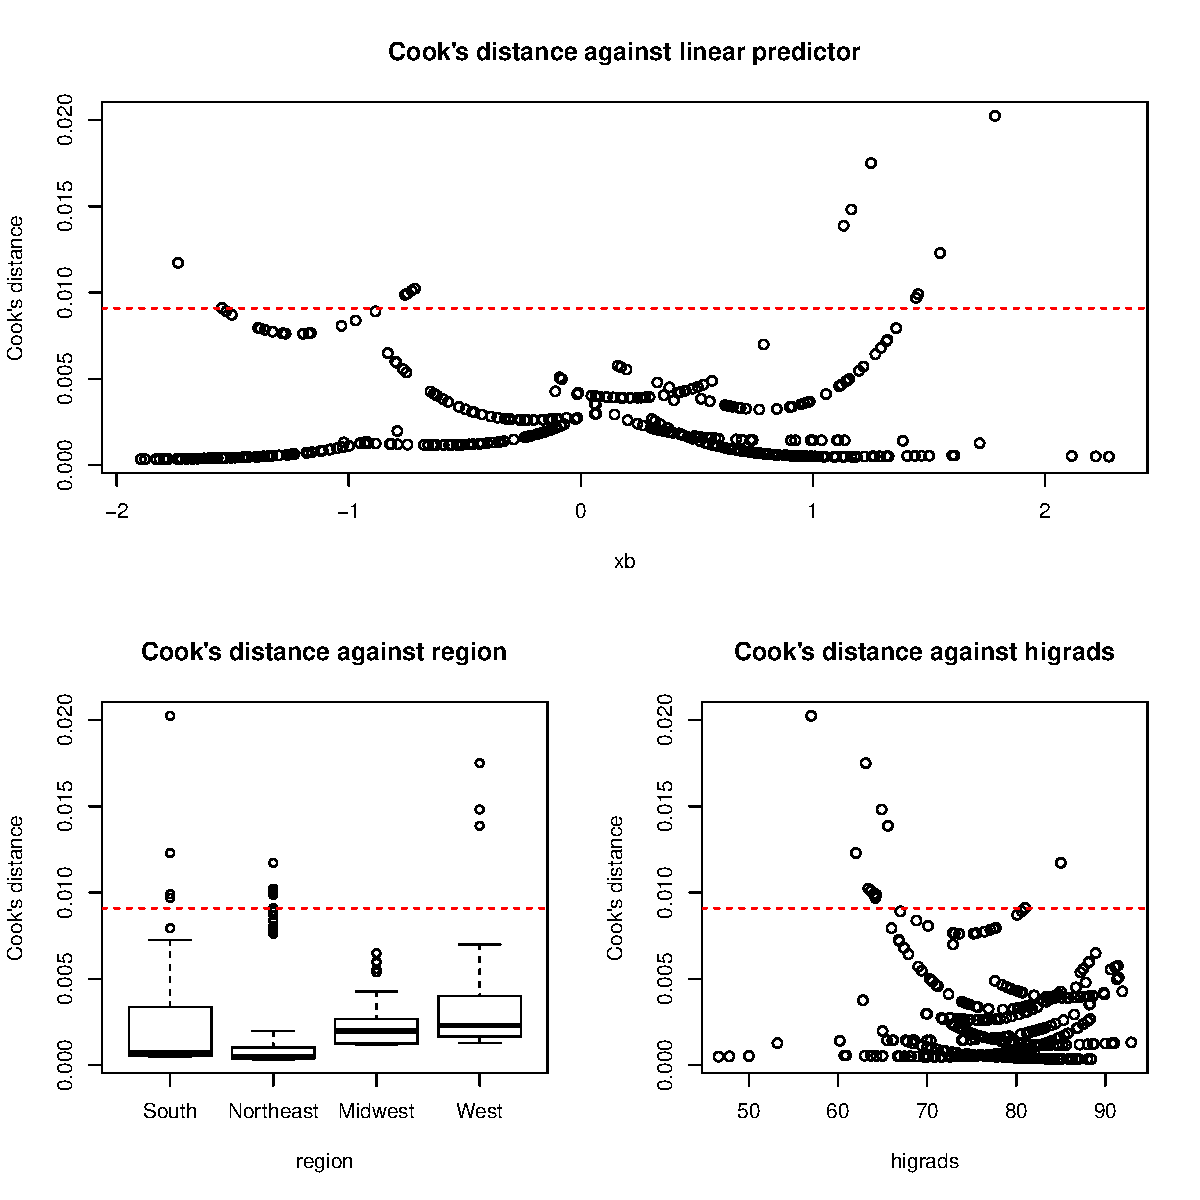
\includegraphics{Project_2_files/figure-latex/unnamed-chunk-12-1} \caption{\label{fig:residuals_combined}Squared standardized Pearson residuals as well as standardized deviance residuals for the combined model, against the linear predictor $x^{\beta}$}\label{fig:unnamed-chunk-121}
\end{figure}
\begin{figure}[h]
\includegraphics{Project_2_files/figure-latex/unnamed-chunk-12-2} \caption{\label{fig:residuals_combined}Squared standardized Pearson residuals as well as standardized deviance residuals for the combined model, against the linear predictor $x^{\beta}$}\label{fig:unnamed-chunk-122}
\end{figure}

For a standardized pearson residual to be considered suspiciously large,
\(|r_i| > |\lambda_{\alpha/2}| ≈ 2\). This is true for 8 of the
standadized pearson residuals, which can be seen in figures XX and XX,
where the standardized pearson residuals are plotted against the linear
predictor. For a deviance residual to be considered to large
\$\textbar{}r\_i\textbar{} \textgreater{} 2 \$. This is never the case
which is verified by figure XX where the standardized devience residuals
are plotted against the linear predictor.

In order to measure how the \(\beta\)-estimates were influenced by
indiviual observations Cook's distance for logistic regression was
calcultaed and plotted.

\begin{figure}[h]
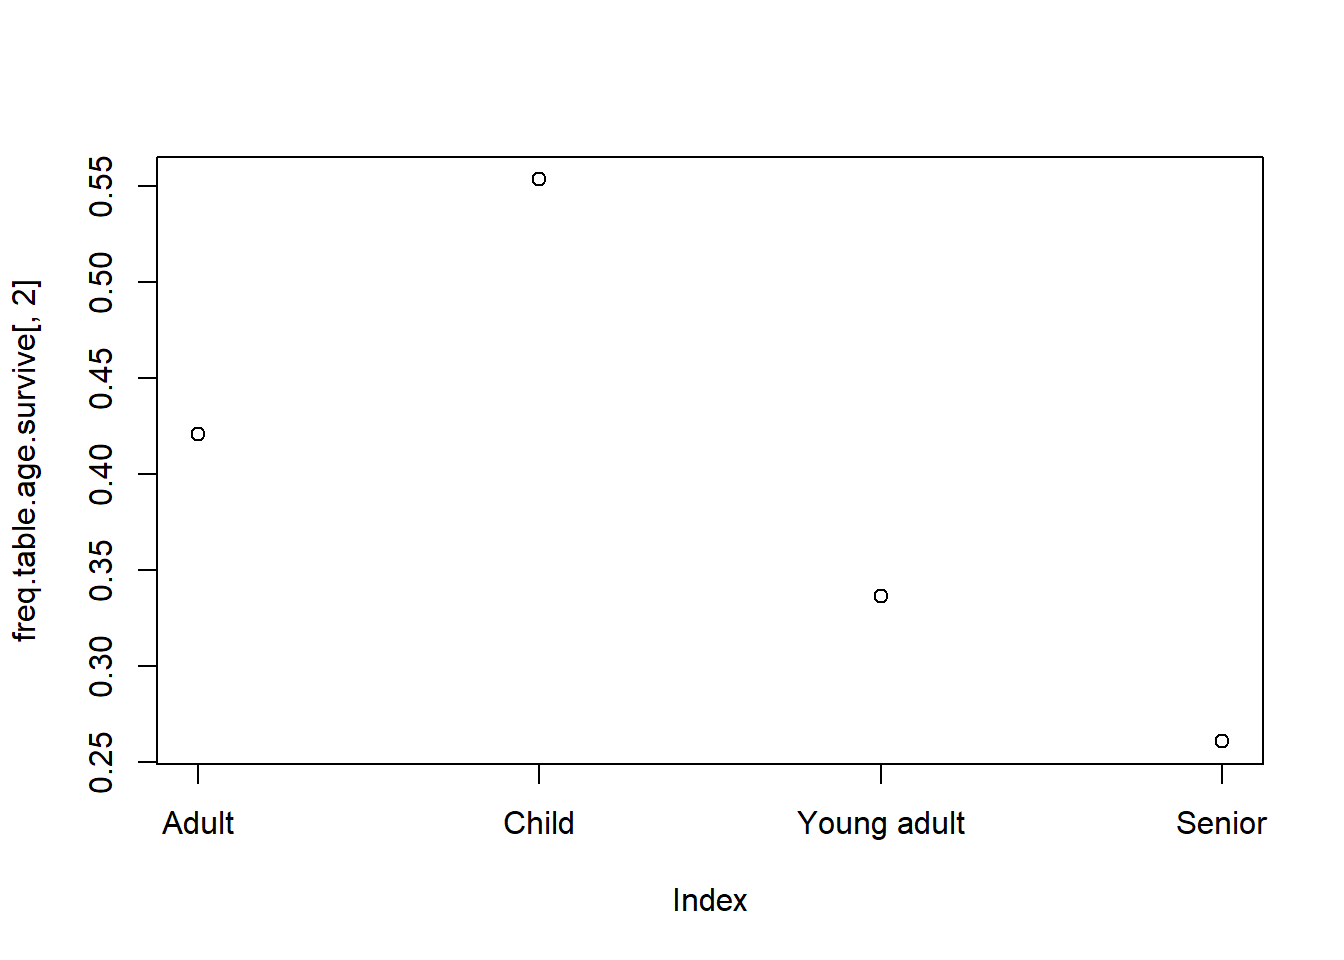
\includegraphics{Project_2_files/figure-latex/unnamed-chunk-13-1} \caption{\label{fig:cooks_combined}Cook's distance, for the combined model, against linear predictor, region as well as higrads}\label{fig:unnamed-chunk-13}
\end{figure}

ANALYS HäR As can be seen in diagrams XX, XX, XX there are several
points over the 4/n thresholds.

Anything alarmin? Any interesting finds?

\hypertarget{interaction-model}{%
\subsection{Interaction model}\label{interaction-model}}

\hypertarget{introduction-4}{%
\subsubsection{Introduction}\label{introduction-4}}

As a forth model, interaction terms are also considered, building in
that the effect of higrads may be different in different regions, where
the log-odds in the model includes interaction terms such as
\(\beta_{Northeast * higrads} \cdot X_{higrads,i}\).

\hypertarget{model-performance}{%
\subsubsection{Model performance}\label{model-performance}}

The performance of the interaction model compared to the combined model
may be analyzed by the likelihood test. This test is similar to a
partial F-test, but adapted for logistical regression, using likelihoods
since sums of squares are not applicable. The likelihood test results in
the interaction model being significantly better than the combined
model, with a P-value of 0.019.

In addition, the AIC, BIC, Nagelkerke, sensitivity and specificity is
compared to the combined model, in table
\ref{tab:compare_sense_spec_interaction}. Performance of the interaction
model can be analyzed by studying a QQ-plot (see figure
\ref{fig:qq-plot_interaction}) the squared standardized Pearson
residuals and the standardized deviance residuals against the linear
predictor \(x^{\beta}\) (see figure \ref{fig:residuals_interaction}). As
well as the Cook's distance against the linear predictor, and against
\texttt{higrads} and against \texttt{region} (see figure
\ref{fig:cooks_interaction}).

\begin{longtable}[]{@{}lrrrrr@{}}
\caption{\label{tab:compare_sense_spec_interaction}Comparison of
sensitivity and specificity of models}\tabularnewline
\toprule
Covariate & AIC & BIC & Sensitivity (\%) & Specificity (\%) & Pseudo
R2\tabularnewline
\midrule
\endfirsthead
\toprule
Covariate & AIC & BIC & Sensitivity (\%) & Specificity (\%) & Pseudo
R2\tabularnewline
\midrule
\endhead
Combined model & 533 & 566 & 72 & 68 & 0.25\tabularnewline
Interaction model & 537 & 558 & 70 & 67 & 0.23\tabularnewline
\bottomrule
\end{longtable}

\newpage

\begin{figure}[h]
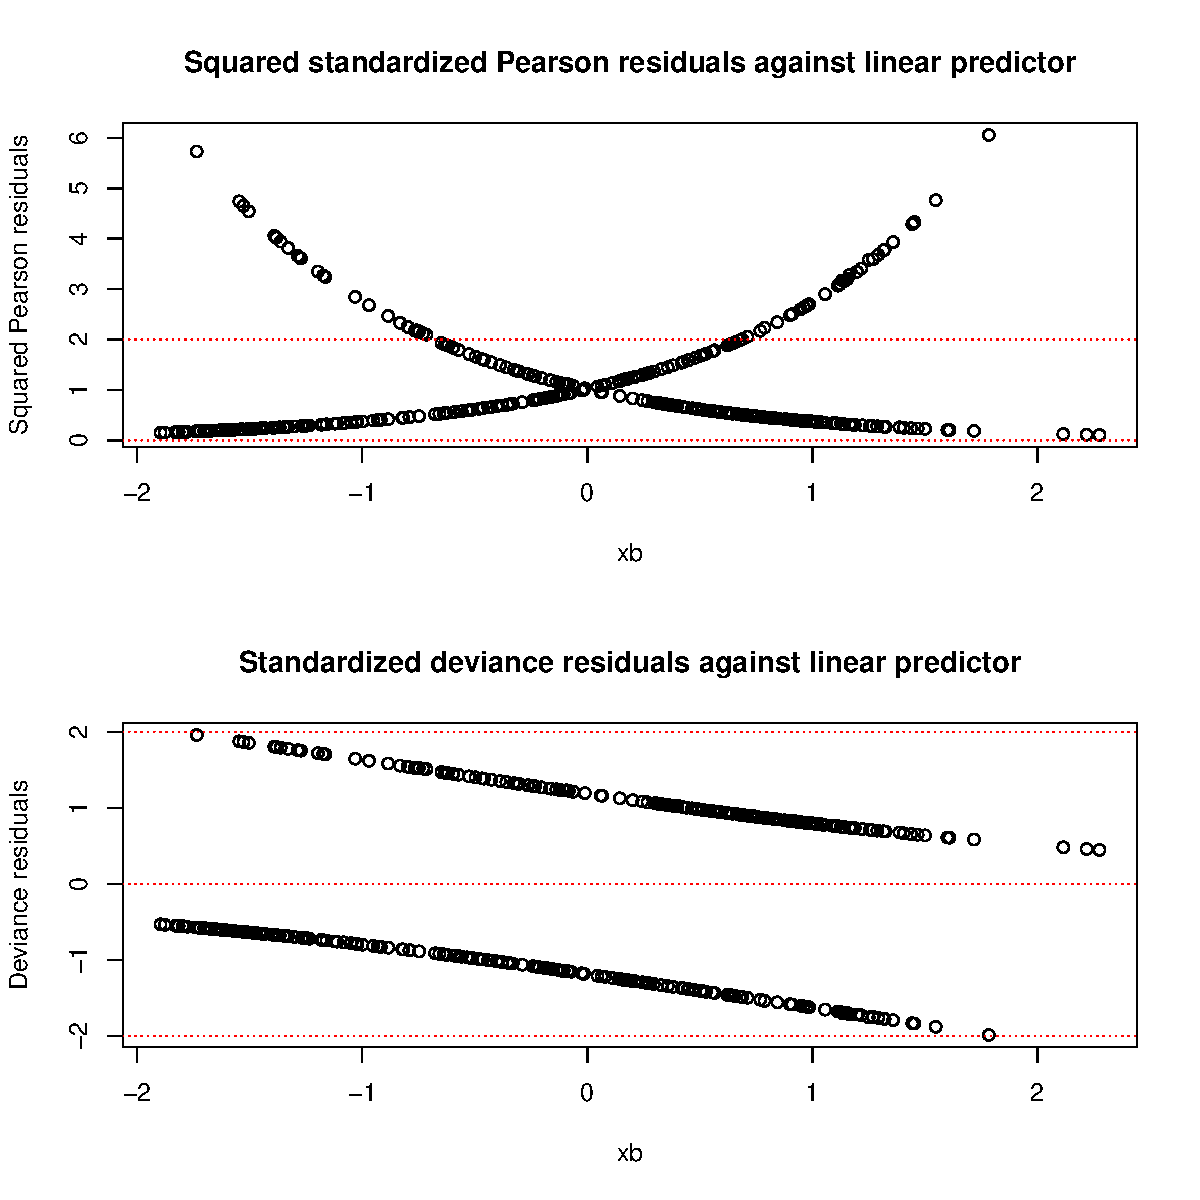
\includegraphics{Project_2_files/figure-latex/unnamed-chunk-16-1} \caption{\label{fig:qq-plot_interaction}QQ-plot for the integration model}\label{fig:unnamed-chunk-16}
\end{figure}

\begin{figure}[h]
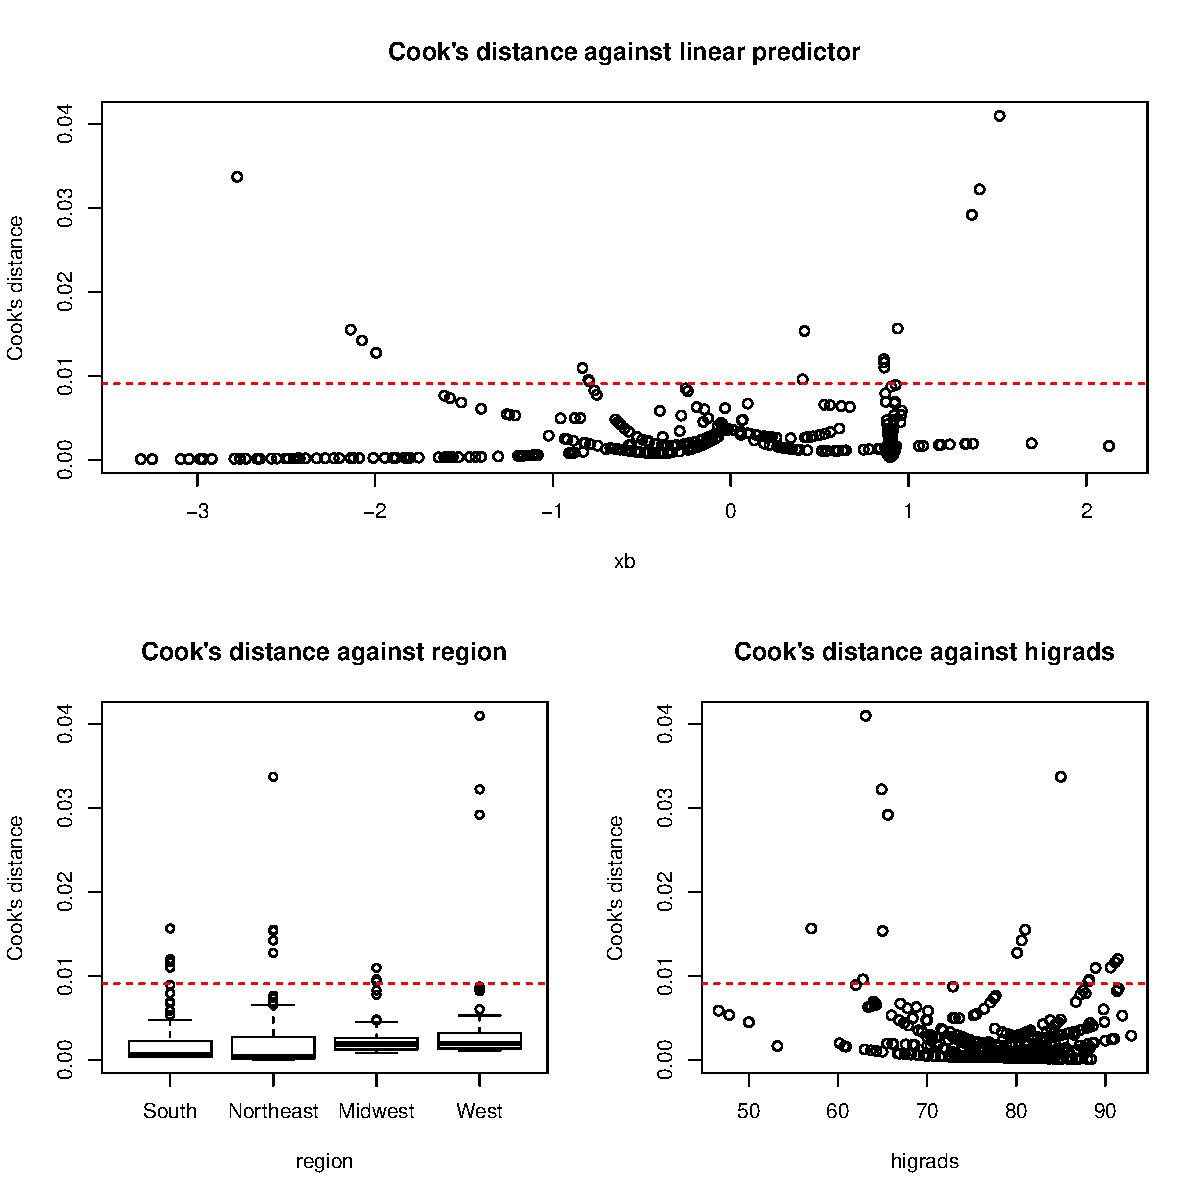
\includegraphics{Project_2_files/figure-latex/unnamed-chunk-17-1} \caption{\label{fig:residuals_interaction}Squared standardized Pearson residuals as well as standardized deviance residuals for the interaction model, against the linear predictor $x^{\beta}$}\label{fig:unnamed-chunk-17}
\end{figure}

\begin{figure}[h]
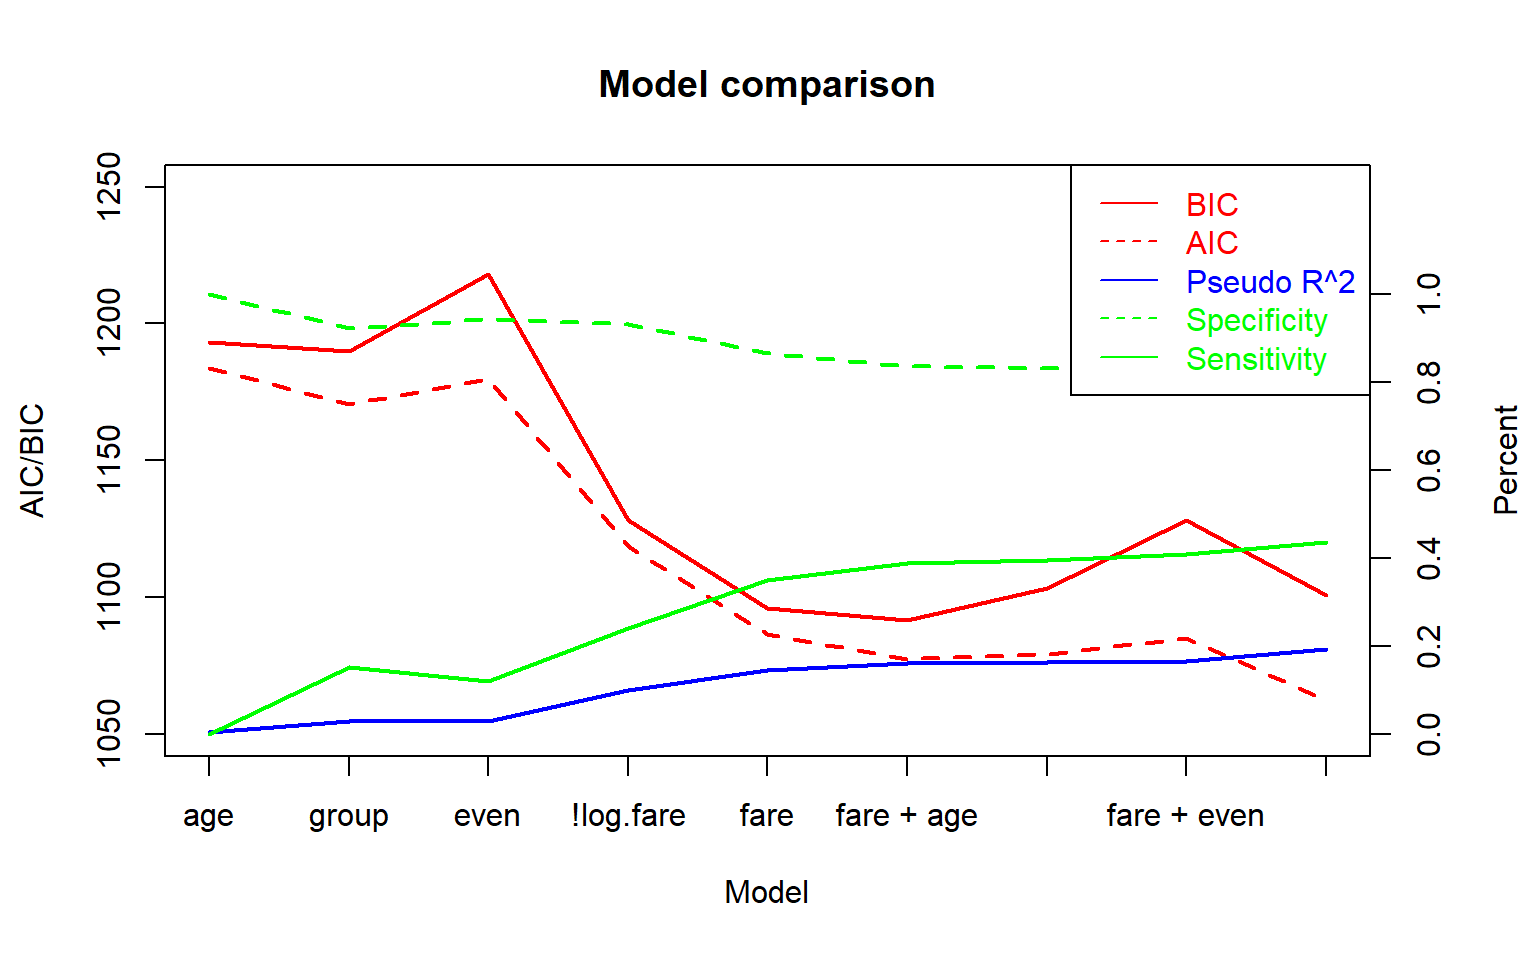
\includegraphics{Project_2_files/figure-latex/unnamed-chunk-18-1} \caption{\label{fig:cooks_interaction}Cook's distance, for the interaction model, against linear predictor, region as well as higrads}\label{fig:unnamed-chunk-18}
\end{figure}

Both models perform better on some metrics, while performing worse on
other. The interaction model has a worse AIC-value, but a lower
BIC-value (KOMMENTERA). The sensitivity, specificity and Pseudo \(R^2\)
values are worse for the interaction model.

NÅGOT OM COOKS MM?

VILKEN ÄR BÄST?

\hypertarget{finding-the-optimal-model}{%
\subsection{Finding the optimal model}\label{finding-the-optimal-model}}

\hypertarget{methology}{%
\subsubsection{Methology}\label{methology}}

Next, an attempt to fit an optimal model to predict high crime rates is
made, using the previous covariates, as well as \texttt{poors} and
\texttt{pshys1000}. Interaction terms are ignored.

Models of increasingly complexity, adding more covariates are compared
to each other on the used metrics, i.e.~AIC, BIC, Pseudo \(R^2\),
sensitivity and specificity. In addition, the result of automatic
selection using R \texttt{step} function is studyied.

\hypertarget{model-comparison-1}{%
\subsubsection{Model comparison}\label{model-comparison-1}}

AIC, BIC and Pseudo \(R^2\) of the studied model are shown in figure
\ref{fig:comparison_optimal}. In addition, table
\ref{tab:comparison_optimal} includes sensitivity and specificity for
the different models.

\begin{figure}[h]
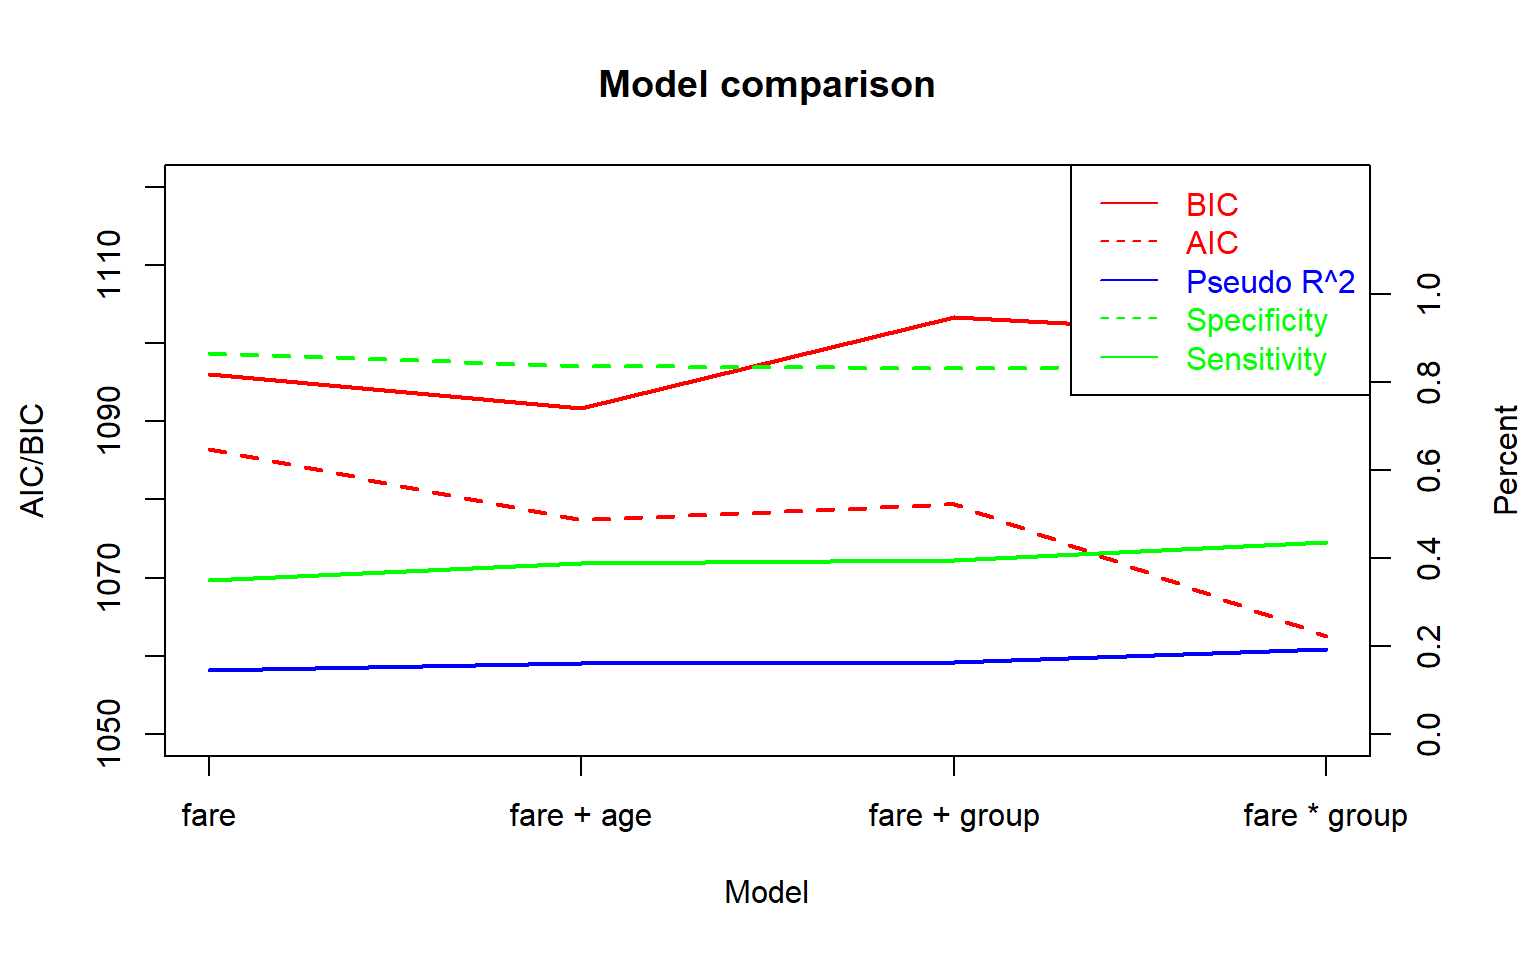
\includegraphics{Project_2_files/figure-latex/unnamed-chunk-20-1} \caption{\label{fig:comparison_optimal}Comparison of AIC and BIC and Nagelkerke psuedo $R^2$ for the different models. Key: H = \texttt{higrads}, R = \texttt{region}, Po = \texttt{poors}, Phy = \texttt{phys1000}}\label{fig:unnamed-chunk-20}
\end{figure}

\begin{longtable}[]{@{}lrrrrr@{}}
\caption{\label{tab:comparison_optimal}Comparison of sensitivity and
specificity of models. Key: H = \texttt{higrads}, R = \texttt{region},
Po = \texttt{poors}, Phy = \texttt{phys1000}}\tabularnewline
\toprule
Model & AIC & BIC & Sensitivity (\%) & Specificity (\%) & Pseudo
R2\tabularnewline
\midrule
\endfirsthead
\toprule
Model & AIC & BIC & Sensitivity (\%) & Specificity (\%) & Pseudo
R2\tabularnewline
\midrule
\endhead
H & 601 & 609 & 55 & 57 & 0.04\tabularnewline
H + R & 537 & 558 & 70 & 67 & 0.23\tabularnewline
H + R + Po & 494 & 518 & 73 & 75 & 0.34\tabularnewline
H + R + Po + Phy & 481 & 509 & 74 & 75 & 0.37\tabularnewline
R + Po + Phy & 480 & 504 & 75 & 74 & 0.37\tabularnewline
H + R + Phy & 508 & 532 & 72 & 72 & 0.30\tabularnewline
\bottomrule
\end{longtable}

The results in \ref{fig:comparison_optimal} and
\ref{tab:comparison_optimal} show that the \texttt{region} +
\texttt{poors} + \texttt{phys1000} model performs best on most of the
metrics. This result is also consistent with the \texttt{step} algorithm
results. As such, this model is considered the \textbf{optimal model}
for this problem.

\hypertarget{model-performance-1}{%
\subsubsection{Model performance}\label{model-performance-1}}

Performance of the optimal model is then analyzed by studying a QQ-plot
(see figure \ref{fig:qq-plot_optimal}) the squared standardized Pearson
residuals and the standardized deviance residuals against the linear
predictor \(x^{\beta}\) (see figure \ref{fig:residuals_optimal}). As
well as the Cook's distance against the linear predictor, and against
\texttt{higrads} and against \texttt{region} (see figure
\ref{fig:cooks_optimal}).

\newpage

\begin{figure}[h]
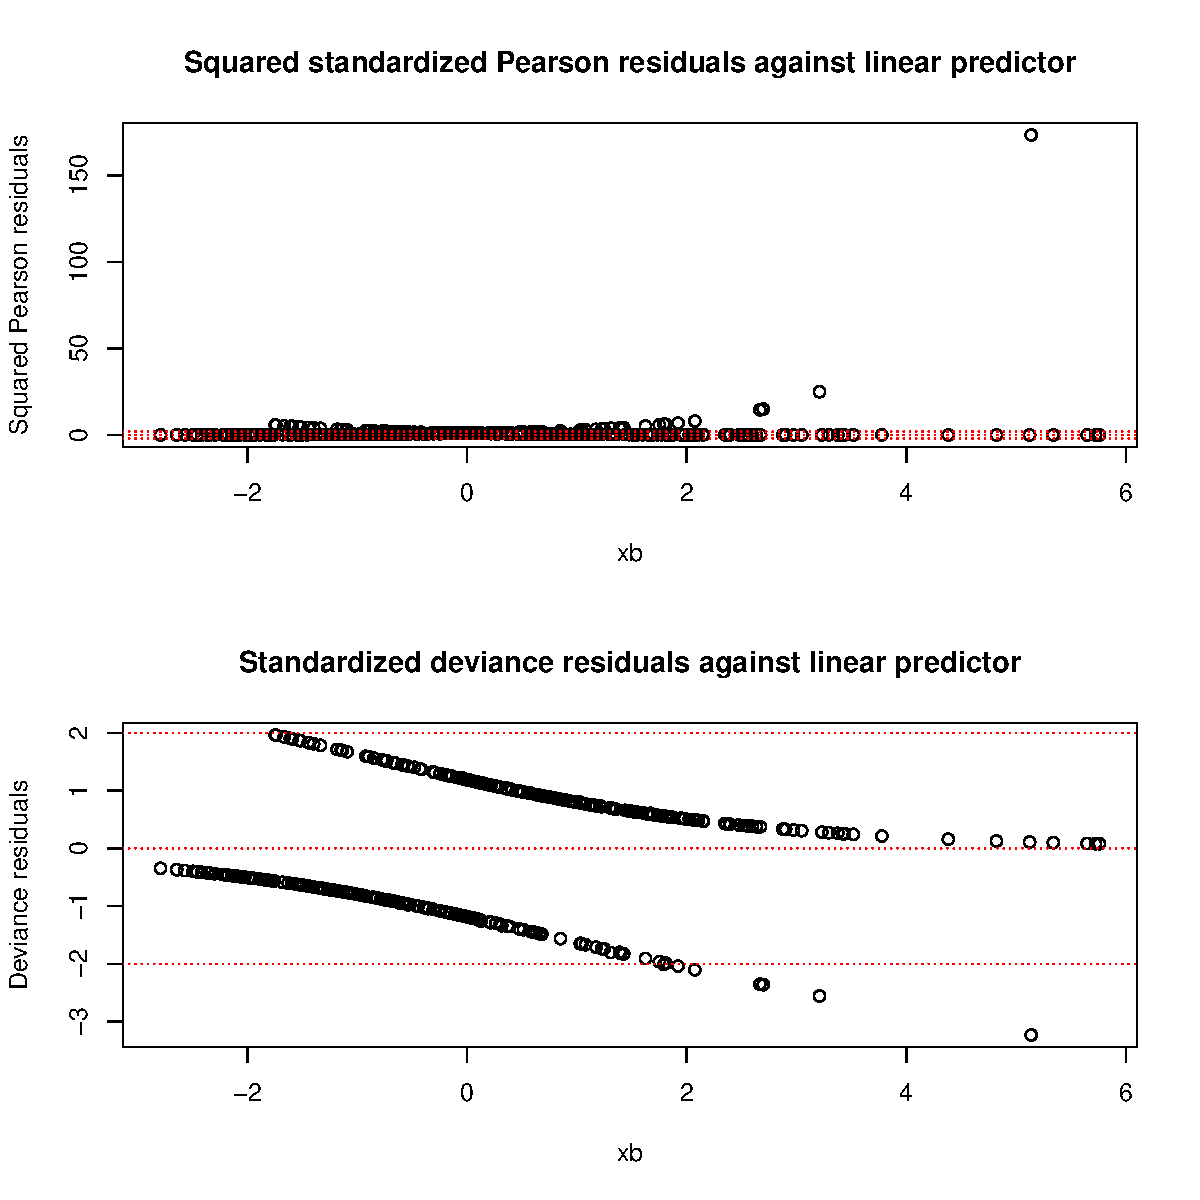
\includegraphics{Project_2_files/figure-latex/unnamed-chunk-23-1} \caption{\label{fig:qq-plot_optimal}QQ-plot for the optimal model}\label{fig:unnamed-chunk-23}
\end{figure}

\begin{figure}[h]
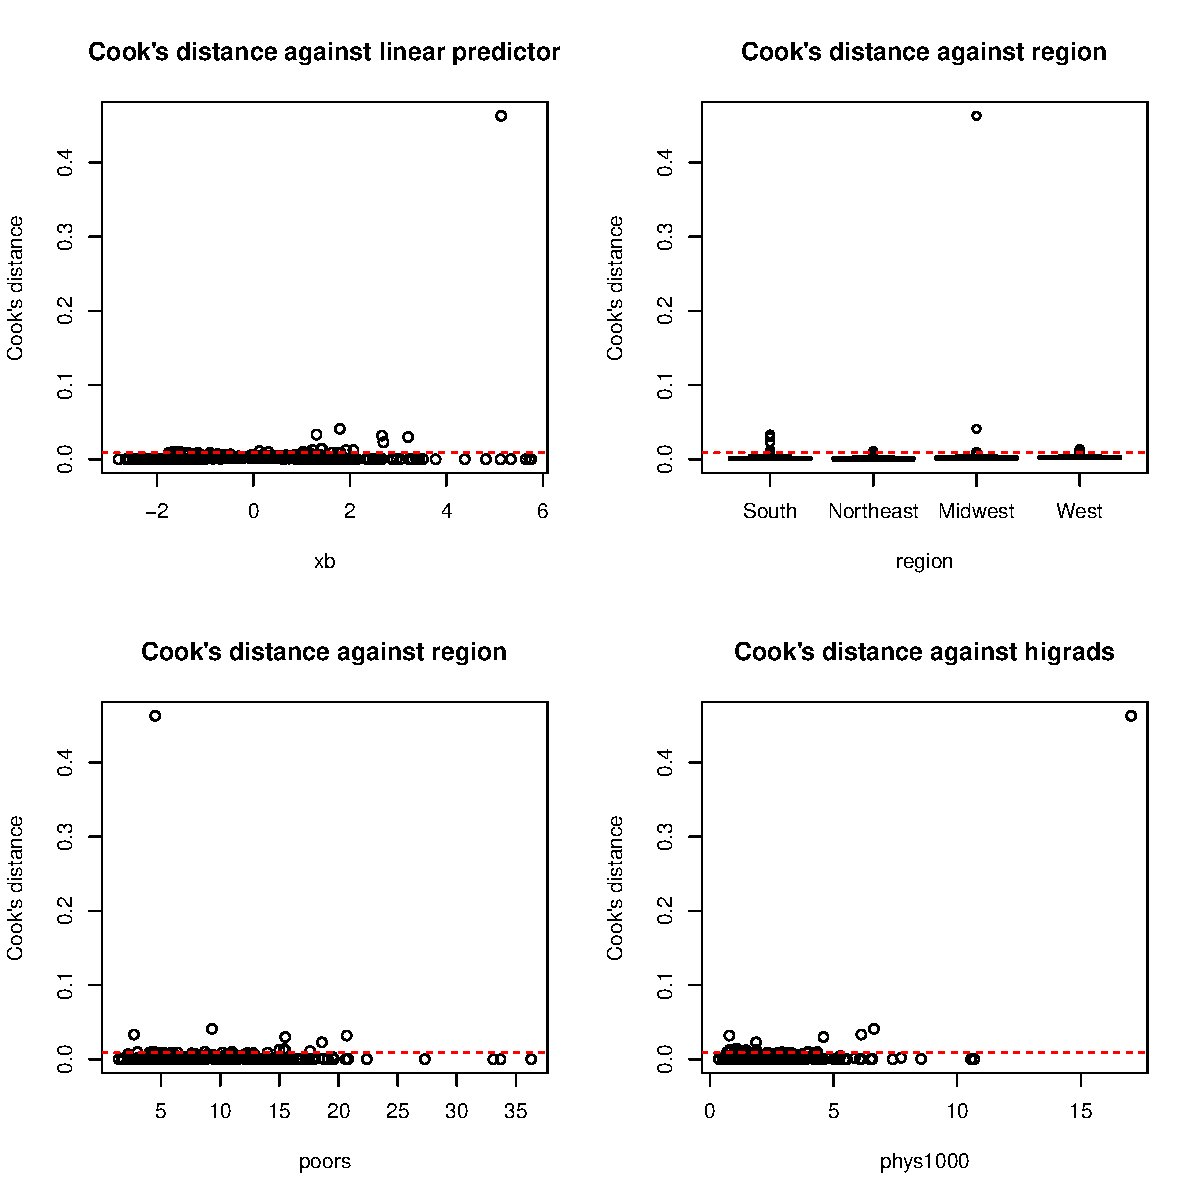
\includegraphics{Project_2_files/figure-latex/unnamed-chunk-24-1} \caption{\label{fig:residuals_optimal}Squared standardized Pearson residuals as well as standardized deviance residuals for the optimal model, against the linear predictor $x^{\beta}$}\label{fig:unnamed-chunk-24}
\end{figure}

\begin{figure}[h]
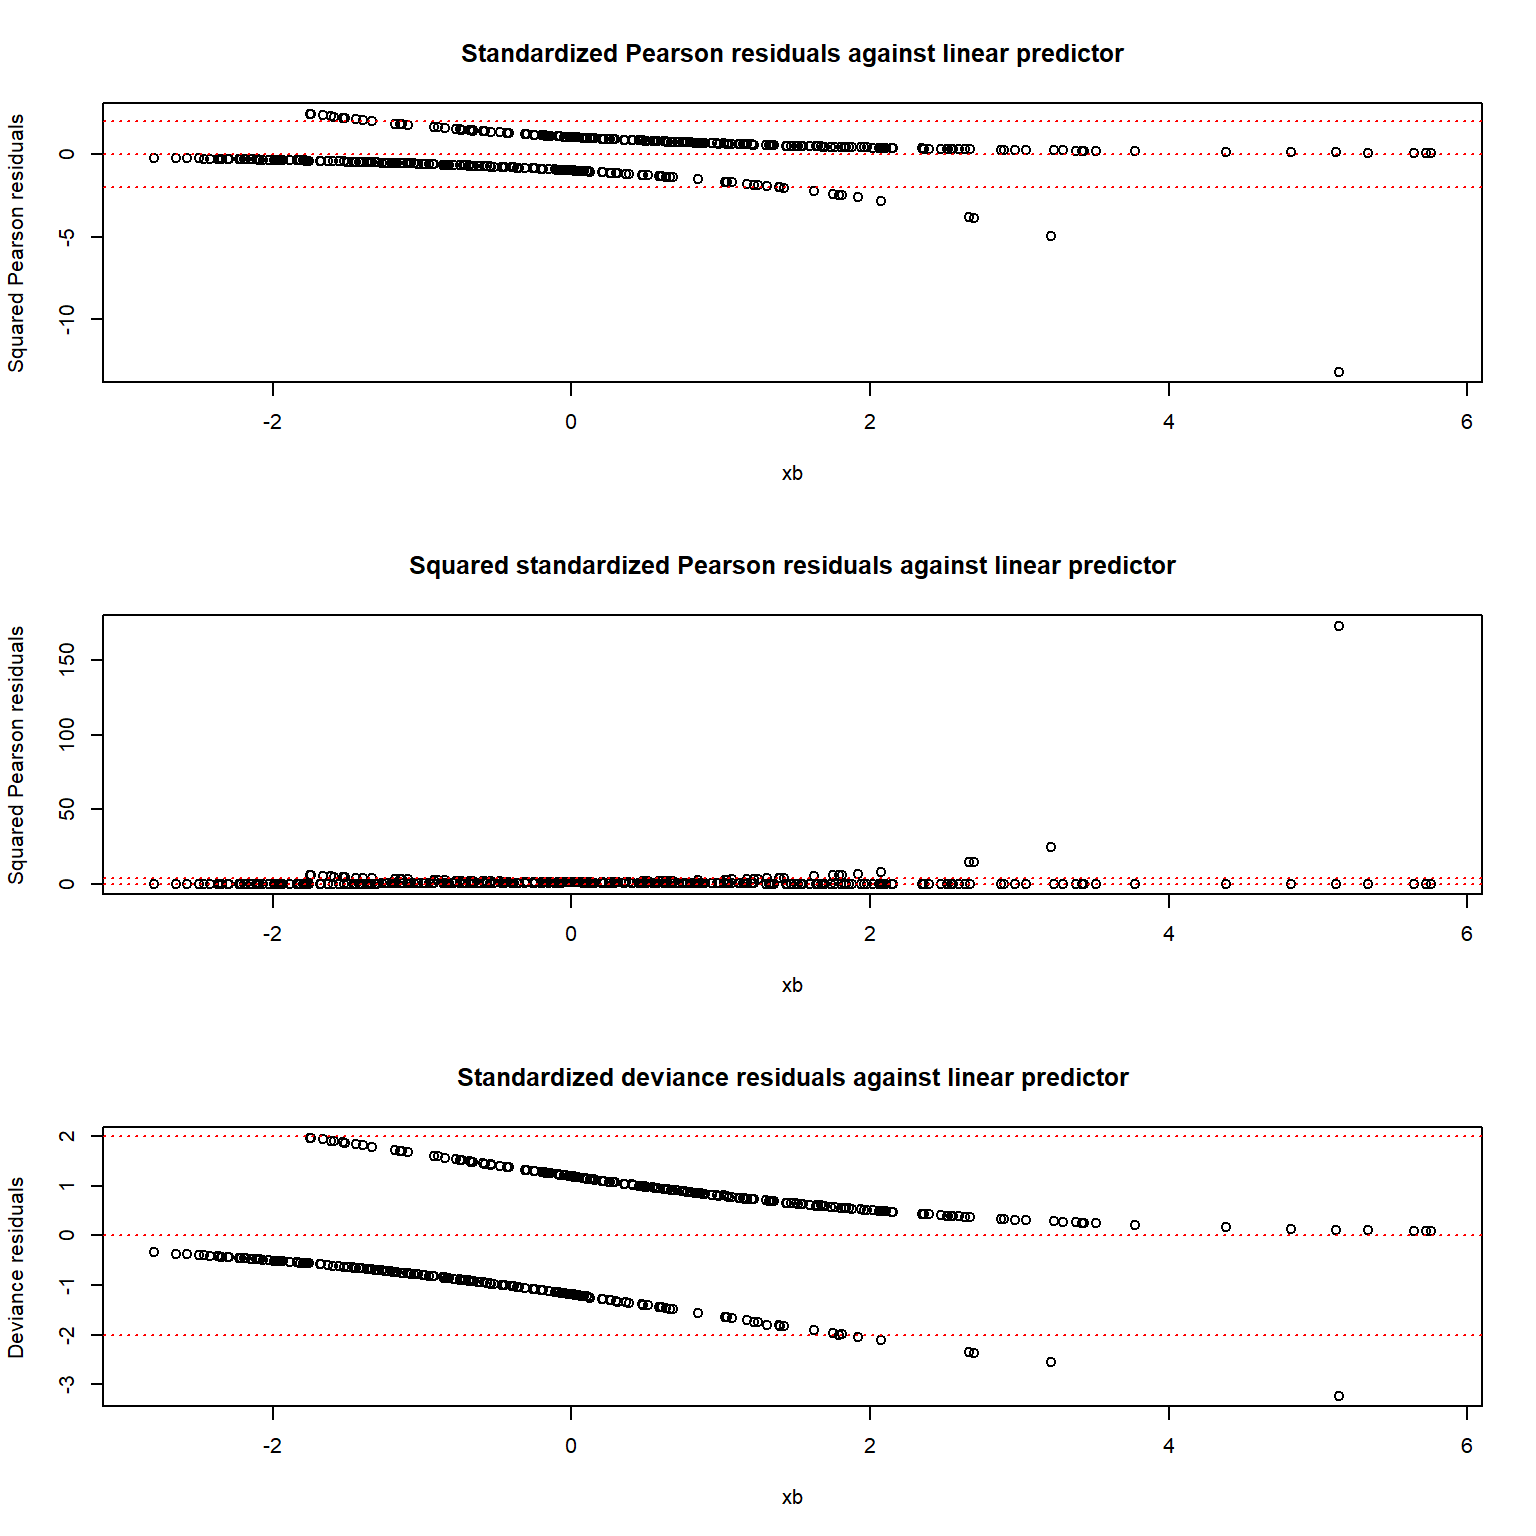
\includegraphics{Project_2_files/figure-latex/unnamed-chunk-25-1} \caption{\label{fig:cooks_optimal}Cook's distance, for the optimal model, against linear predictor, region as well as higrads}\label{fig:unnamed-chunk-25}
\end{figure}

The outlier is Olmsted

\hypertarget{discussion}{%
\subsubsection{Discussion}\label{discussion}}

In order to first get a view on the different covariates and how they
relate to each other, they are plotted against eachother in figure
\ref{fig:pairs}.

\begin{figure}[h]
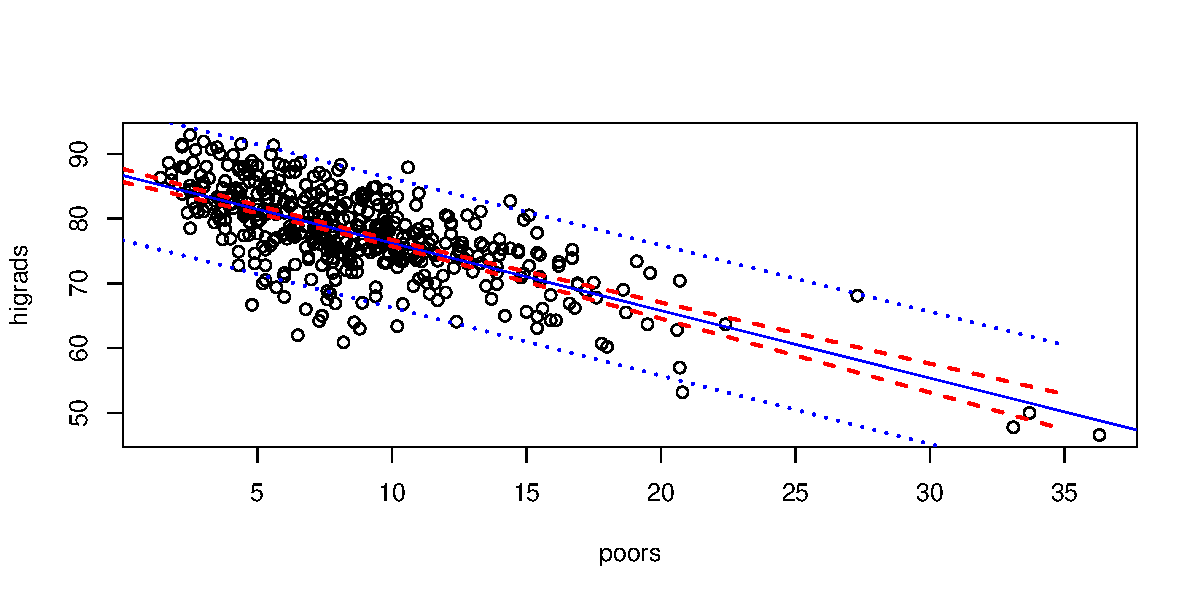
\includegraphics{Project_2_files/figure-latex/unnamed-chunk-27-1} \caption{\label{fig:pairs}Plot of covariates against eachother}\label{fig:unnamed-chunk-27}
\end{figure}

The optimal model includes the previously studied covariate
\texttt{region}, but discards the \texttt{higrads} covariate. In
addition, it includes the new \texttt{poors} and \texttt{phys1000}
covariates. One explaination why \texttt{higrads} is not used in the
optimal may be seen in figure \ref{fig:pairs}, where there seems to be a
high correlation between \texttt{higrads} and \texttt{poors}.

This hypothesis is tested in figure \ref{fig:poors_higrads}, where a
linear regression model has been fit. Studying the P-value of the model
reveals that the \(\beta\)-values are highly significant.
\textbackslash{}begin\{figure\}{[}h{]}
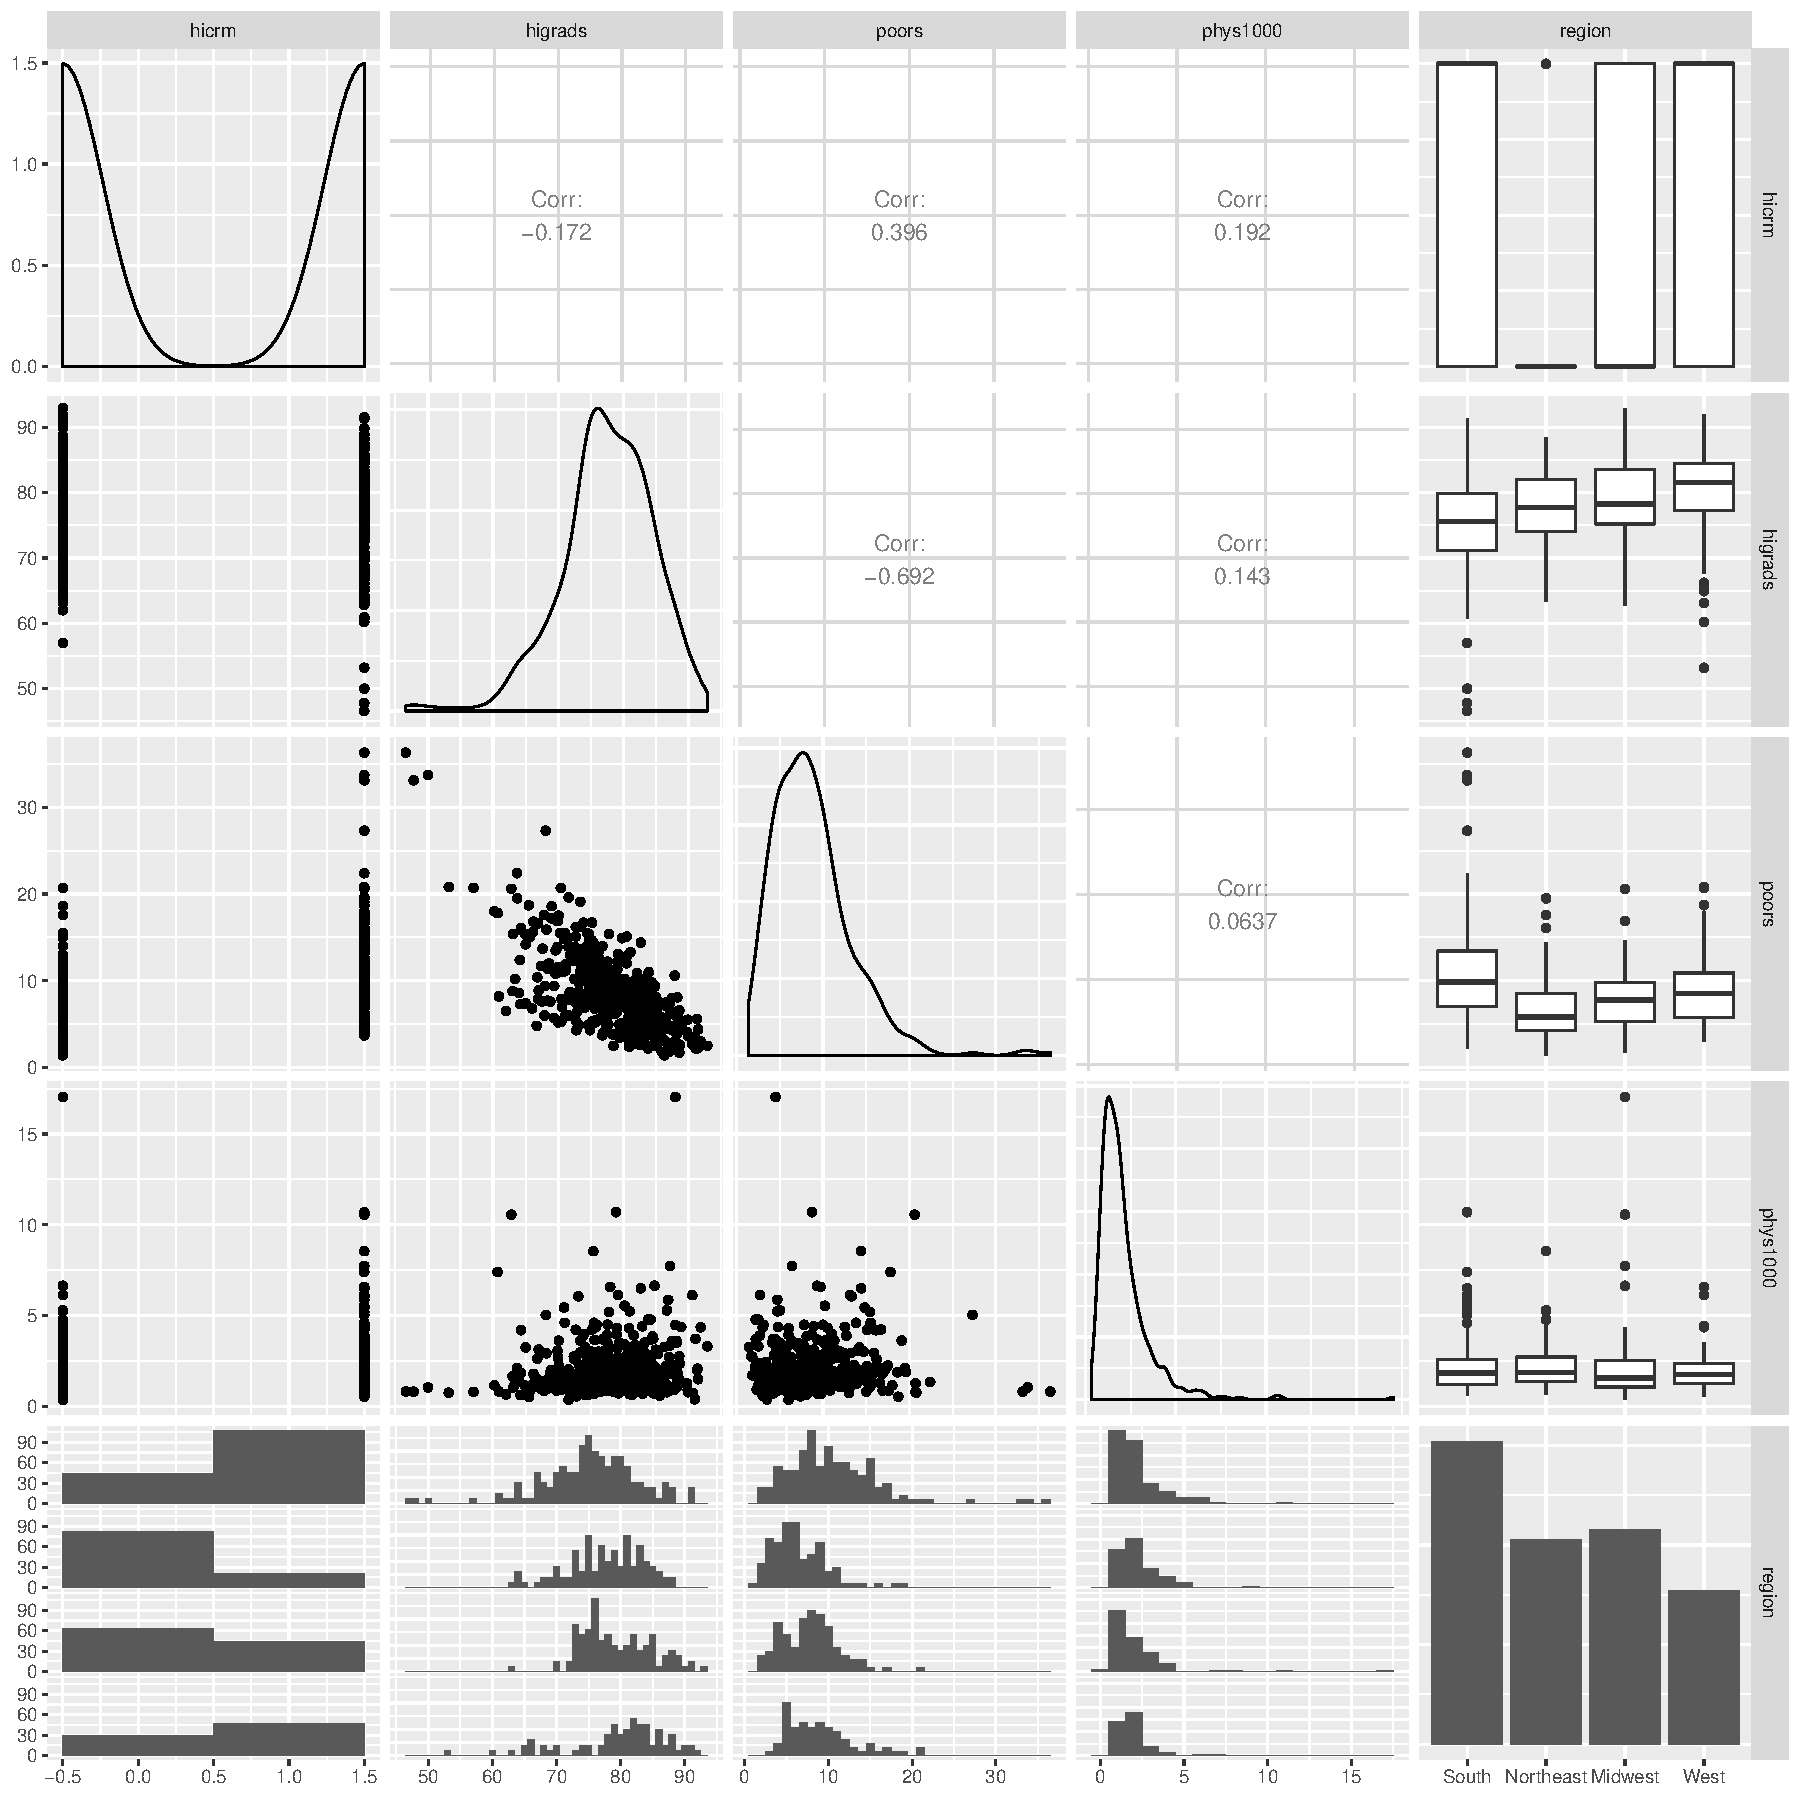
\includegraphics{Project_2_files/figure-latex/unnamed-chunk-28-1}
\textbackslash{}caption\{\label{fig:poors_higrads}Plot of
\texttt{higrads} against \texttt{poors}, together with linear regression
line, with 95 \% confidence and prediction
intervals\}\label{fig:unnamed-chunk-28} \textbackslash{}end\{figure\}

Looking at how well \texttt{poors} predicts \texttt{hicrm} may be seen
in figure \ref{fig:hicrm_poors}. Here it may be seen that \texttt{poors}
follow a more distinct S-shape, and that \texttt{poors} seems to split
the dataset more distinctly between high and non-high crime rate, as it
varies from \(\approx 15% - \approx 80%
\), rather than the low separation discussed previously. As such,it
seems that \texttt{higrads} and \texttt{poors} are highly correlated,
but that \texttt{poors} better predict \texttt{hicrm} and is therefore
better left in the model.

\begin{verbatim}
#> 
#> Call:
#> glm(formula = hicrm ~ poors, family = "binomial", data = cdi)
#> 
#> Deviance Residuals: 
#>     Min       1Q   Median       3Q      Max  
#> -2.4611  -0.9885  -0.2648   1.0397   1.6873  
#> 
#> Coefficients:
#>             Estimate Std. Error z value Pr(>|z|)    
#> (Intercept) -2.04623    0.27545  -7.429 1.10e-13 ***
#> poors        0.24276    0.03126   7.765 8.14e-15 ***
#> ---
#> Signif. codes:  0 '***' 0.001 '**' 0.01 '*' 0.05 '.' 0.1 ' ' 1
#> 
#> (Dispersion parameter for binomial family taken to be 1)
#> 
#>     Null deviance: 609.97  on 439  degrees of freedom
#> Residual deviance: 526.19  on 438  degrees of freedom
#> AIC: 530.19
#> 
#> Number of Fisher Scoring iterations: 4
\end{verbatim}

\begin{figure}[h]
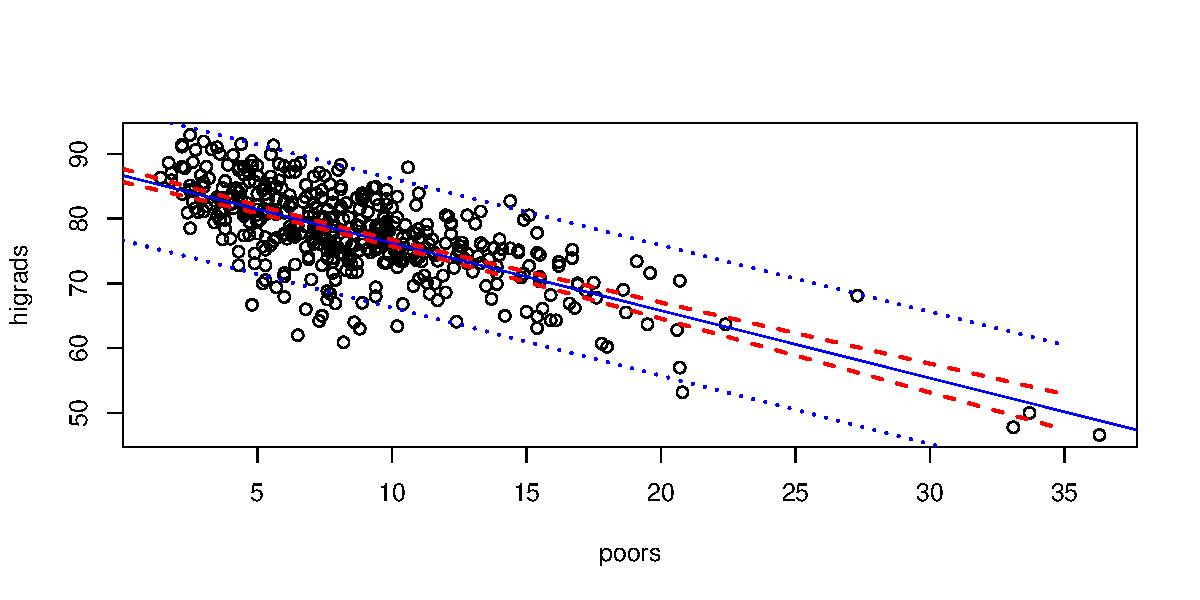
\includegraphics{Project_2_files/figure-latex/unnamed-chunk-29-1} \caption{\label{fig:hicrm_poors}Plot of \texttt{hicrm} against \texttt{poors}, including kernel smoothing and prediction of fitted model with 95 \% confidence interval}\label{fig:unnamed-chunk-29}
\end{figure}

Regarding \texttt{phys1000}, it appears in \ref{fig:pairs} that it does
not have an as clear relationship to the other covariates and therefore
provides more information to the model. Looking at how well
\texttt{phys1000} predicts \texttt{hicrm}, seen in figure
\ref{fig:hicrm_phys1000}, it seems to follow an approximate S-shape and
therefor contributes to the model.

\begin{verbatim}
#> 
#> Call:
#> glm(formula = hicrm ~ phys1000, family = "binomial", data = cdi)
#> 
#> Deviance Residuals: 
#>     Min       1Q   Median       3Q      Max  
#> -3.1344  -1.0989  -0.3058   1.1853   1.3977  
#> 
#> Coefficients:
#>             Estimate Std. Error z value Pr(>|z|)    
#> (Intercept) -0.67608    0.19474  -3.472 0.000517 ***
#> phys1000     0.32757    0.08466   3.869 0.000109 ***
#> ---
#> Signif. codes:  0 '***' 0.001 '**' 0.01 '*' 0.05 '.' 0.1 ' ' 1
#> 
#> (Dispersion parameter for binomial family taken to be 1)
#> 
#>     Null deviance: 609.97  on 439  degrees of freedom
#> Residual deviance: 591.10  on 438  degrees of freedom
#> AIC: 595.1
#> 
#> Number of Fisher Scoring iterations: 4
\end{verbatim}

\begin{figure}[h]
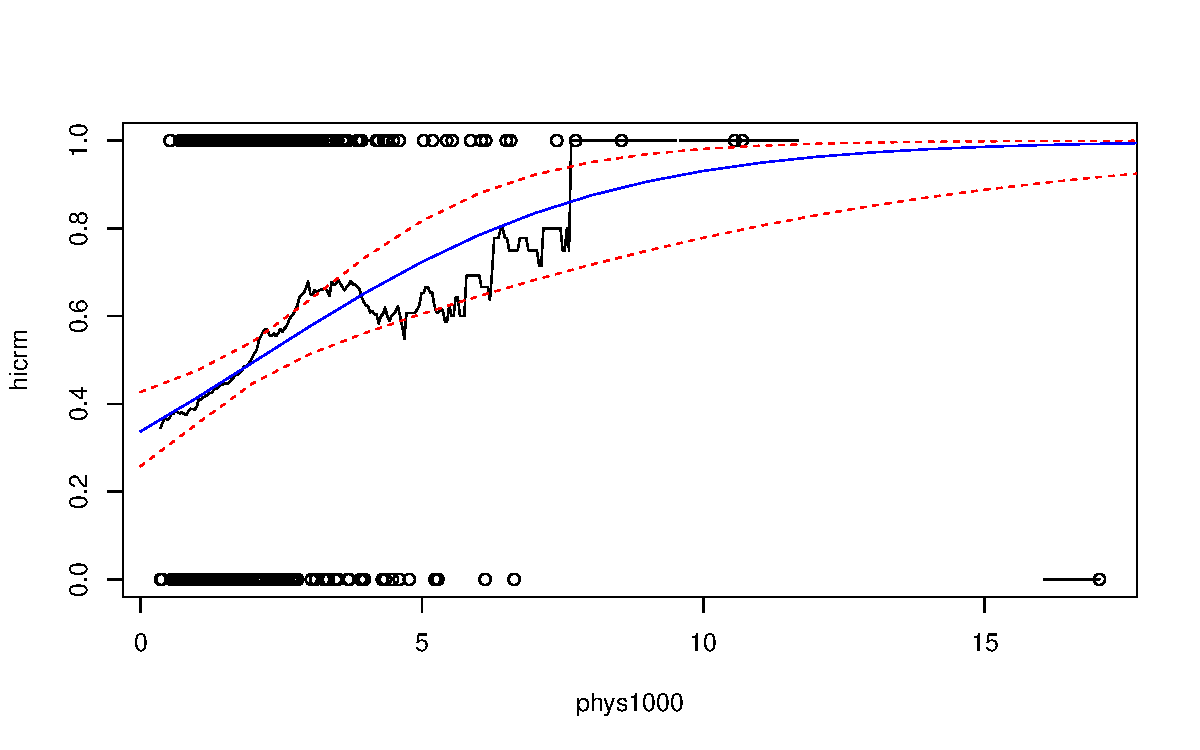
\includegraphics{Project_2_files/figure-latex/code_plot-1} \caption{\label{fig:hicrm_phys1000}Plot of \texttt{hicrm} against \texttt{phys1000}, including kernel smoothing and prediction of fitted model with 95 \% confidence interval}\label{fig:code_plot}
\end{figure}


\end{document}
